\chapter{Survey of the Literature}\label{chap:literature_review}
In this thesis, we aim to unify the rich dynamics of gaze during active visual search within a single physics-inspired model, deepening our understanding of the neural computations underlying search behaviour. This approach draws on the growing success of methods from statistical physics and nonlinear dynamics in computational neuroscience, particularly in characterising the complex spatiotemporal activity of neural circuits. Applying a similar perspective to gaze trajectories, we seek to identify common dynamical principles across spatial and temporal scales.

In \cref{sec:gaze_traj}, we review the background for developing a scientific understanding of the dynamics of visual gaze; the data we present in this thesis, the unique spatiotemporal patterns of such data, and the previous methods used to model complex dynamics found in gaze trajectories are each described. In \cref{sec:diffusive_processes}, we introduce the theoretical framework of stochastic modelling, Lévy motion, and the anomalous superdiffusion found elsewhere in complex dynamical systems. \cref{sec:comp_sampling} then links stochastic dynamics to computational sampling, in both biological and abstract contexts, and provides the key motivation for developing a mathematical understanding of a gaze trajectory as a proxy for dynamical attention in the brain. 

%%% 1.3 Behavioural Data
\section{Gaze trajectories}
\label{sec:gaze_traj}
%To ground the physical background of this thesis, the present section reviews the physical system we aim to model: the eye-tracking signal which characterises human visual attention. During active vision, the visual system does not operate as a passive receiver of sensory input, but rather as an active, dynamic sampler of a changing environment \cite{friston_does_2018, friston_sophisticated_2021}. This active sensing manifests across two coupled physical observables: the internal dynamics of rich neural oscillatory networks, and the external, mechanical execution of gaze trajectories. Crucially, these domains inform and drive each other, and each exhibit complex, scale-free dynamics in their activity. Characterised by background spectra with power law tails and anomalous diffusion, the visual system is capable of devoting attention to many spatiotemporal scales of event. Viewing these biological phenomena through the lens of statistical mechanics provides a rigorous foundation for mathematically modelling the visual system. This section establishes these empirical constraints by first examining the functional role of neural frequency bands and theta-gamma coupling (\cref{subsec:neur_freq_bands}), before detailing the multi-scale, stochastic regimes of human gaze trajectories (\cref{subsec:gaze_traj}). Together, these behavioural patterns motivate the fractional dynamics given by the FNS equations of motion, and the developments upon that model in the subsequent sections.
Healthy human gaze trajectories are well characterised by a small set of dynamical patterns, the challenge is in understanding their interaction, functional roles, and mechanistic origin. The clearest pattern of gaze trajectories is a division into long jumps in positional attention called saccades, between which are periods of relative stillness called fixations during which information is gathered \cite{erkelens_coordination_2006, seung_how_1996, lencastre_dynamical_2025, benitezy_eyetracking_1970}. Eye-tracking devices---such as the Eyelink 1000 used in collecting data for this thesis as shown in \cref{fig:eye-tracking}\textbf{d)}---provide the high-precision measurements to analyse and model the gaze trajectories through continuous time, both during saccade and fixation.

%This paradigm has a limited history in the literature, and fitting data to a simple jump process called a Lévy flight (see \cref{subsec:levy_motion}) parameterised by the stable parameter $\alpha$ has found some limited use as a biomarker for ADHD \cite{papanikolaou_levy_2024}. Broader saccade metrics based on such jump processes have been found to be valuable as non-invasive biomarkers for broader neural disorders, including schizophrenia \cite{caldani_saccadic_2017, morita_eye_2017, zhu_diagnosis_2024, lindner_disorders_2005, zhu_diagnosis_2024}, autism \cite{bittencourt_saccadic_2013, wang_saccadic_2025}, ADHD \cite{papanikolaou_levy_2024}, and Parkinson's disease \cite{wang_saccadic_2025, bittencourt_saccadic_2013, kaski_ocular_2017}. 

\begin{figure}[b!]
	\centering
	\begin{subfigure}[T]{0.2\textwidth}
		\centering
		\includesvg[width=\linewidth]{figures/schematics/head-schematic-1}
	\end{subfigure}
	\hfill
	% \begin{subfigure}[T]{0.18\textwidth}
	% 	\centering
	% 	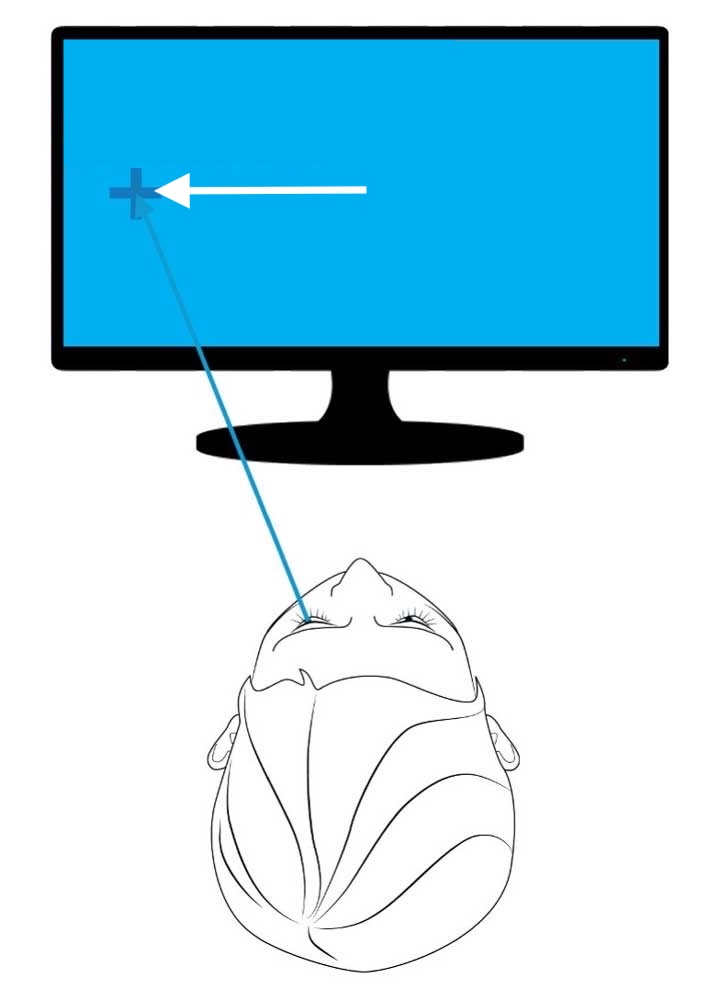
\includegraphics[width=\linewidth]{figures/schematics/head-2.jpg}
	% 	\label{subfig:gamma_fits}
	% \end{subfigure}
	\begin{subfigure}[T]{0.2\textwidth}
		\centering
		\includesvg[width=\linewidth]{figures/schematics/head-schematic-2}
	\end{subfigure}
    \hfill
	\begin{subfigure}[T]{0.2\textwidth}
		\centering
		\includesvg[width=\linewidth]{figures/schematics/head-schematic-3}
	\end{subfigure}
    \hfill
    \begin{subfigure}[T]{0.3\textwidth}
		\centering
		\includesvg[width=\linewidth]{figures/schematics/head-schematic-4}
	\end{subfigure}
	\caption{\textbf{A schematic representation of a typical eye-tracking setup.} \textbf{a)} shows a subject at the beginning of a typical eye-tracking study, with gaze position starting at the centre of the screen $(960, 540)$~\unit{\px}. \textbf{b)} shows a saccade from the centre towards the left of the screen as a target is tracked. \textbf{c)} shows the return of gaze position to the centre of the screen, as the target returns to the centre. \textbf{d)} shows a typical eye-tracking unit, the EyeLink 1000 Plus, as used in the experiment studied in this thesis.\textit{\textbf{a)}--\textbf{c)} are adapted from \cite{srresearch2020eyelink3}, while \textbf{d)} is adapted from \cite{srresearch2013eyelink1000plus}}}
	\label{fig:eye-tracking}
\end{figure}

Where the dynamics of fixation or gaze have been considered, they are treated as separate subject matter to each other, and rarely treated together in single studies. Gaze fixations exhibit three distinct dynamical patterns: near-instant microsaccades within the same point of focus, slow ocular drift about a point of focus, and high frequency ocular micro tremor \cite{van_ede_looking_2026,graham_ocular_2023, engbert_integrated_2011, spauschus_origin_1999}. There are a number of studies examining a rich physical model of fixational dynamics \cite{engbert_integrated_2011, engbert_normal, vasudevan_stochastic_nodate}, as well as developing the role such dynamics have in gathering information efficiently \cite{rucci_control_2015, rucci_miniature_2007, rucci_temporal_2018, rucci_unsteady_2015, roberts_fixational_2013, wu_fixational_2024}.

\subsection{Existing models of visual searching dynamics}\label{subsec:existing_models}
Progress towards modelling gaze dynamics during visual search spans physics, neuroscience, and machine learning. As such, existing models have been built with very different aims and methods. Cognitive and biologically inspired models explain where attention is drawn through biologically-inspired saliency maps and top-down guidance \cite{itti_model_1998, wolfe_guided_2021, Gayet2025-fv}. More normative models ask what an optimally informative searcher would do, selecting saccades by Bayesian belief updating and entropy reduction \cite{najemnik_optimal_2005}. We here examine in detail two influential models representing these two model-making paradigms, those being the self-avoiding random walk model of fixational dynamics presented in \cite{engbert_integrated_2011, Herrmann2017-hw}, and DeepGaze~III from \cite{kummerer_deepgaze_2022} which utilises a deep learning model to predict saccade positions. A full comparison of a selection of influential and successful models, along with a comparison of their core domains, aims, and key features, is given in \cref{tab:search_models_colored} in \cref{app:prior_models}.

The self-avoiding random walk presented in \cite{engbert_integrated_2011} considers the dynamics within a single quadratic potential which confines the gaze into a localised fixation. The gaze position is discretised on a square lattice, and visited positions will increase potential to introduce a self-avoidance condition, which relaxes on a short timescale. Of particular interest to this thesis is the interpretation of the explored potential as a motor map from the neurons in the superior colliculus to motivate a physics-inspired model of gaze \cite{doi:10.1126/science.1166112, CARPENTER2000R291, Sparks2002-zb}. The self-avoidance condition, although taking a different motivation, is mechanistically very similar to the kernel adaptation which we introduce in this thesis to explain rhythmicity in global saccade timings. This work successfully reproduces superdiffusion in fixations, alongside the existence of microsaccades. This model, however, only accounts for fixational motion, and does not aim to capture the long saccades which organise them. Further, although the authors mention tremor, a tremor-frequency peak is not observed in this model.

DeepGaze~III \cite{kummerer_deepgaze_2022} produces fixation prediction through a state-of-the-art deep convolutional neural network, a map of observed oculomotor biases (such as an observed centre-bias in viewing an image), and a history of previous fixations, to predict the location of saccades with the highest accuracy to-date across all metrics considered in the standard MIT/Tübingen Saliency Benchmark \cite{mit-tuebingen-saliency-benchmark, kummerer_deepgaze_2022}. This model is highly successful in fixation prediction, and has been used to research patterns in attention through simulation of saccade prediction without requiring human measurement, however it lacks biological or functional usefulness beyond fixation position. The model provides no temporal information, only providing the location of fixations, and does not consider the dynamics of fixations themselves, nor providing any mapping from biologically realistic neural activity onto the dynamics of gaze.

\subsection{Timescales of neural computation}\label{subsec:neur_freq_bands}
Throughout much of this thesis, links are drawn between model dynamics and well-studied frequency bands of activity in the human brain. It is then valuable to outline the studied computational and functional interpretations of such frequency bands. Neural firing activity is divided into frequency bands named by greek letters, originally discovered and decomposed from electroencephalogram (EEG) data \cite{fan_relation_2007, klimesch_frequency_2018}. Divisions are only approximate, but bands may be thus considered: delta (\SIrange{0.1}{3}{\hertz}), theta (\SIrange{4}{8}{\hertz}), alpha (\SIrange{8}{14}{\hertz}), beta (\SIrange{14}{40}{\hertz}), and gamma (\SIrange{40}{100}{\hertz}) \cite{fan_relation_2007, klimesch_frequency_2018}. Of particular interest to this thesis are the interpretations of theta and gamma neural activity as functionally important to neural computation. Broadly, theta rhythms have been found to modulate and organise bursts in computational gamma-scale neural activity  \cite{qi_fractional_2022, fries_mechanism_2005, fries_rhythmic_2023, fries_rhythms_2015, spyropoulos_theta_2018, bastos_communication_2015}. Theta rhythms have been shown to modulate attention during auditory tasks \cite{wang_attention_2022, yang_neural_2024}, visual search tasks \cite{kawashima_attentional_2022, spyropoulos_theta_2018, Mo_competing_2019}, and when analysing the broad attentional mechanism of the brain \cite{tan_theta_2024, fan_relation_2007, klimesch_frequency_2018}. 

Theta-rhythmic cycles are finding strong interpretation in the cognitive neuroscience literature as organising and communicating information sampled from the environment for integration into the internal model of the brain \cite{fries_mechanism_2005, fries_rhythmic_2023, fries_rhythms_2015, spyropoulos_theta_2018, bastos_communication_2015}. Strong direct evidence for this theory include correlations between intelligence and high theta peak power in EEG data during tasks requiring focus and attention \cite{wang_attention_2022, tan_theta_2024}, and the discovered sensitivity of the visual system to react and search scenes on a theta rhythm \cite{kawashima_attentional_2022, spyropoulos_theta_2018}. Accordingly, the firing patterns which define the lowest level of computation carried out in the brain are regularly found to be gamma in timescale, with broadband signals being found within \SIrange{40}{100}{\hertz} in a wide range of measurements of neural activity during cognitive tasks \cite{canolty_high_2006, harris2026-cn, ursino_thetagamma_2024, brooks_thetagamma_2020, tort_thetagamma_2009}. The coupling between the phase of theta activity and the amplitude of gamma activity is known as theta-gamma coupling (TGC). This phenomenon, a specific form of phase-amplitude coupling (PAC), is schematically represented in \cref{fig:litrev-thetagamma_coupling}. The evidence and theory behind TGC are described in a systematic review by \textcite{ursino_thetagamma_2024}. This thesis provides a computation view of the function of TGC the within the search dynamics of gaze as modulating periods of fixational attention on a slow theta-scale, during which information is dynamically sampled on a gamma scale. 
\begin{figure}[h!]
	\centering
	\includegraphics[width=0.75\linewidth]{figures/Theta_Gamma_Coupling_image.pdf}
	\caption{\textbf{A schematic representation of theta-gamma coupling (TGC).} Here, neural population patterns $\textbf{A}-\textbf{E}$ are activated in sequence on the timescale of a gamma oscillation $f>30\text{Hz}$, triggered by the phase of a modulating theta wave of neuron population \textbf{T} on the theta timescale of $4-8 \text{Hz}$. Such a formulation of TGC as correctly ordering signals has its foundations in the work of \textcite{lisman_theta-gamma_2013}, and was subsequently expanded to describe the dynamic neural mechanism during sensory exploration to modulate close attention upon individual centres of focus \cite{mclelland_theta-gamma_2016}. \textit{Schematic adapted from Figure.~2 of \textcite{ursino_thetagamma_2024}}}
	\label{fig:litrev-thetagamma_coupling}
\end{figure}

%%% 1.1 Statistical physics
\section{Diffusive processes}\label{sec:diffusive_processes}
In formalising empirical observations of human gaze and neural activity into a mathematical model, this thesis relies on the framework of non-equilibrium statistical mechanics and stochastic calculus. When a system is driven by a massive number of microscopic interactions—such as the complex interconnected firing of a neural population—modelling the exact deterministic dynamics becomes intractable. Instead, statistical physics provides the tools to coarse-grain these high-dimensional systems into low-dimensional stochastic differential equations. This section establishes the mathematical progression necessary to model scale-free visual inference. We first review the classical paradigm of normal diffusion and Brownian motion (\cref{sec:brownian_motion}), which serves as the foundational model for standard diffusive physical systems. We then examine how systems of interest frequently violate the classical assumptions of normal diffusion and Brownian motion, leading to an understanding of the presence and role of anomalous diffusion in many complex dynamical systems (\cref{subsec:anom_diff}). Finally, we introduce Lévy stable motion (\cref{subsec:levy_motion}), a class of superdiffusive fractional stochastic processes that mathematically capture the heavy-tailed, intermittent dynamics characteristic of optimal visual search and neural activity.
\subsection{Brownian motion and normal diffusion}\label{subsec:brownian_motion}
Statistical modelling has been fundamental in understanding complex dynamical systems: separating the dynamics of macroscopic observables into deterministic terms and stochastic terms reduces chaotic high-dimensional systems to a small number of variables of interest \cite{hassler_stochastic_2016, cunchala2024basicoverviewvariousstochastic}. Stochastic processes are often the most natural, tractable, and accurate modelling tools when examining high-dimensional chaotic systems across physics, economics, geology, climate science, machine learning, and neuroscience \cite{[CITE]}. The universality of these stochastic models is understood to be an implication of the central limit theorem: the distribution of the summed effect of a large number of identical and independently distributed (i.i.d) random variables of finite mean and variance will approach a Gaussian \cite{ulyanov2024classical, heyde1978central, gnedenko1954limit}. The technique of treating a large number of independent coupled deterministic variables as a single stochastic variable turns out to be generalisable to a wide class of problems involving coupled, non-stationary, or diverging-variance processes which are out of equilibrium, such as in the case of neuronal spiking patterns \cite{18k5-pwl1, La_Camera_2022_meanfieldneuron}. The most ubiquitous stochastic process is central to statistical physics: the Brownian motion $W_t$, equivalently called the Wiener process, which consists of stationary and independent Gaussian increments across all non-overlapping time intervals. The Brownian motion is a very simple and analytically robust model of the coarse-grained effect of a high dimensional system of contributions which are flattened to a small number of observable dimensions. A Brownian motion is defined only by its timescale, with a variance over trajectories after time $t$ of $t$ itself. Realisations of Brownian motion yield time series' which are almost surely continuous but nowhere differentiable. Classical examples of processes modelled by the Brownian motion are: the movement of a macroscopic particle in a non-turbulent fluid \cite{hassler_stochastic_2016}, the gravitational influence of an orbiting collection of stars on supermassive black holes \cite{Chandrasekhar1943, Merritt2007a}, and (arguably) the movement of low-volatility stock prices \cite{cunchala2024basicoverviewvariousstochastic}. The generalisation of the Brownian motion for heavy-tailed i.i.d variables is a Lévy flight, and is described in detail in \cref{subsec:levy_motion}, and \cref{fig:brownian_vs_levy} compares the two processes.

To include random variables such as Brownian motion in dynamical systems, physicists and mathematicians have developed the tools of stochastic calculus. Brownian motion of a variable $\textbf{x}_t$ through time $t$ about a potential landscape $V(\textbf{x})$ can be described in terms of the first order Langevin equation:
\begin{equation}\label{eq:langevin}
    d\textbf{x}_t = -\gamma \nabla V(\textbf{x}_t) dt + \sqrt{2 \gamma} dW_t 
\end{equation}
where the constant $\gamma$ describes the noise strength of the Brownian motion \cite{smoluchowski1906zur, langevin1908theorie, uhlenbeck1930theory, kramers1940brownian} and $dW_t$ is a Brownian motion. Although the dynamics of $\textbf{x}_t$ is described stochastically, the dynamics of the corresponding probability distribution $P(\textbf{x},t)$ is deterministic and can be described exactly. Such an equation of motion of $P(\textbf{x},t)$ under any stochastic dynamics defining $\textbf{x}_t$ is called the Fokker-Planck equation \cite{boffi_probability_2023, jordan_variational_1998, wang1945theory, kolmogoroff1931analytischen, planck1917ueber, fokker1914mittlere}. In the case of \cref{eq:langevin}, the Fokker-Planck equation is \cite{jordan_variational_1998, boffi_probability_2023, planck1917ueber}
\begin{equation}\label{eq:overdamped-fokkerplanck}
    \partial_t P(\textbf{x},t) = \frac{\gamma}{2} \nabla \cdot \left( P(\textbf{x},t) \nabla V(\textbf{x}) + \nabla P(\textbf{x},t) \right)
\end{equation}
whose unique stationary distribution is the Boltzmann-Gibbs distribution
\begin{equation}\label{eq:boltzmann-gibbs}
    \pi(\textbf{x}) \propto \exp[-V(\textbf{x})]
\end{equation}
which yields the important relationship, where a 
Langevin potential can be constructed from a normalised target density via $V(\textbf{x}) = -\ln \pi(\textbf{x})$, which we will make use of in this thesis in constructing saliency maps from empirical data where only the likelihood of fixations $\pi(\textbf{x}))$ is given. %Importantly, the dynamical system defined by \cref{eq:langevin} is ergodic, and thus under \cref{eq:overdamped-fokkerplanck}, any initial distribution will converge to $\pi(\textbf{x})$. 
Importantly, the Langevin system Fokker-Planck equation \ref{eq:overdamped-fokkerplanck} will describe the diffusion of a sharply peaked initial distribution as it widens, and the statistics of this diffusion from a sharp initial condition define normal diffusion as follows. The solution to the Fokker-Planck equation from an exact initial condition $P(\textbf{x},0) = \delta^n(\textbf{x}-\textbf{x}_0)$ is dominated over short times by the $\nabla P$ term as $\nabla P \gg P \nabla V$, reducing the Fokker-Planck equation to the heat equation $\partial_t P = \frac{\gamma}{2}\nabla^2 P$. As such, the leading-order short-time solution is that of such a heat equation
\begin{equation}\label{eq:normal_diffusion}
    P(\textbf{x}, \Delta t) \propto \exp \left[ -\frac{\|\textbf{x} - \textbf{x}_0 \|^2}{2(\gamma \Delta t)}\right] \implies \text{Var}[\textbf{x}(\Delta t)] = \gamma \Delta t
\end{equation}
which demonstrates the interesting behaviour which defines normal diffusion: the short-time scaling of variance in position will be linear, as $\text{Var}[\textbf{x}_{\Delta t}] = \gamma \Delta t$. Thus $\gamma$ is often called the timescale of the Brownian motion, as it defines the rate of linear diffusion of variance with time. This linear scaling of the variance of trajectories with time defines normal diffusion \cite{klafter_anomalous_2005, vilk_strong_2025, sposini_towards_2022, oliveira_anomalous_2019}, and understanding those systems whose random motion does not reproduce such normal diffusion is crucial in understanding complex dynamical diffusion.
% The Fokker-Planck equation for the standard Brownian-Langevin system is a diffusion PDE equivalent to the heat equation with a gradient term, a correspondence well-understood before the development of stochastic calculus. The diffusion arising from such small uncorrelated perturbations of a dynamical system leads to the statistical properties which first drove the study of statistical physics, such as normal diffusion and the universality of Brownian motion, which we follow in \cref{subsec:anom_diff} and \cref{subsec:levy_motion} respectively, however the neural system described in this thesis diverges strongly from the Brownian paradigm, requiring an understanding of fractional processes.

% \subsubsection{Further stochastic models}
% Only recently have the universality of stochastic processes asides from the Brownian motion been well-studied. Of interest to this thesis is the case where microscopic perturbations become correlated and yield heavy-tailed statistics. Correlated steps, long-time memory effects, and chaotic microscopic dynamics can result in a stochastic process which does not limit to a Brownian motion \cite{Brevitt2025, Klages2013}. Of interest to us is the fractional \textit{Lévy flight}, a process driven by scale-free noise which span across many orders of magnitude. For instance, a spiking neural network at with diverging activity correlation length, where the centre of mass of neural firing is then subject to large jump discontinuities \cite{La_Camera_2022_meanfieldneuron, qi_fractional_2022, qi_fractional_2022}. Such large jumps in time series' are modelled with to Lévy stable noise, where the increments are drawn independently from a heavy-tailed distribution. This section describes the analytics, stability, and behaviour of such Lévy processes for our current study, and how their diffusive properties differ from the behaviour of Brownian motion.

\subsection{Anomalous diffusion}\label{subsec:anom_diff}
The universality of normal diffusion in systems which are driven by Brownian motion as above has been studied closely, most influentially as in the movement of particles in a fluid \cite{Einstein1905, klafter_anomalous_2005, metzler_anomalous_2014, Merritt2007a}. These dynamics inform the definition of normal diffusion through this variance scaling with time, rigorously calculated as the mean squared displacement (MSD) $\langle \|\Delta \textbf{x} (\Delta t) \|^2 \rangle \propto 
\Delta t$. To study the universality of such normally diffusive processes, the continuous time random walk (CTRW) model was developed, in which a trajectory has subsequent step sizes and durations drawn from finite variance distributions. Such models will universally reproduce this normal diffusive scaling property of $\langle \| \Delta \textbf{x} (t) \| \rangle \propto t$, and as a result of the central limit theorem, will approach Brownian motion. However, increasingly interesting physical systems have been found which diffuse nonlinearly in time, a situation known as anomalous diffusion, with an MSD scaling as:
\begin{equation}
    \langle \| \Delta \textbf{x} (\Delta t) \|^{2} \rangle \propto \Delta t^{\lambda_2}, \ \ \lambda_2 \neq 1
\end{equation}
Such anomalous diffusion yields two cases, subdiffusion $0 < \lambda_2 < 1$ where diffusion scales slower than normal, and superdiffusion $1 < \lambda_2 < 2$ where diffusion scales faster than normal. The case of $\lambda_2 = 2$ is known as ballistic diffusion, as it is found in the deterministic case of constant velocity $x = vt$. An important phenomenon often found in diffusive processes is fractal self-similarity. A Brownian motion is self-similar across all scales, and is nowhere smooth,  and in physical systems demonstrating anomalous diffusion, self-similarity resulting from criticality is often reported. Later in \cref{subsec:levy_motion}, we will find that it is advantageous in the study of anomalous superdiffusion to capture this multi-scale diffusive self-similarity through an extension of the $\lambda_2$ scaling of MSD to a spectrum of absolute moments $\lambda(q)$ which describes the diffusive self-similarity which unifies across many scales of study. A comparison of Brownian motion and Lévy motion which displays their self-similar properties and diffusive scaling through the mean absolute displacement $\langle \|\Delta \textbf{x}\| \rangle \propto \Delta t^{\lambda_1}$ is shown in \cref{fig:brownian_vs_levy}.

Anomalous subdiffusion has been shown to result from heavy-tailed wait-times between interactions \cite{klafter_anomalous_2005}, such as in trapped fluid flow \cite{Kirchner2000-kf}, controlled diffusion through cell membranes \cite{klafter_anomalous_2005}, and protein mixing \cite{Kou2004-kz}. 
\subsubsection*{Anomalous superdiffusion}\label{subsubsec:anomalous_superdiffusion}
Of great importance in studying the dynamcs of visual search, superdiffusion has been studied in the contexts of complex exploratory biological systems. We model the efficient exploration of gaze dynamics through Lévy superdiffusion, which is the standard dynamical model of superdiffusion in physics and is presented in detail in \cref{subsec:levy_motion}. Such Lévy superdiffusion has a strong link to the problem of designing a strategic search for scarce resources. However the true computational benefit of superdiffusion has become a subject of debate in the literature. On one side, the Lévy foraging hypothesis posits that the standard superdiffusive CTRW, the Lévy walk, is an optimal strategy when searching for sparse and randomly distributed resources. On the other, researchers have proposed that such a model is biologically unrealistic and a result of artificial modelling conditions. 

The finding that Lévy superdiffusion is optimal in random search was first reported in a letter to the journal Nature in 1999 by \textcite{viswanathan_optimizing_1999}. In the original paper proposing the Lévy foraging hypothesis a Lévy walk with superdiffusion $\langle x(t) ^2 \rangle \propto \frac{t^2}{\ln(t)}$ on the transition to ballistic diffusion was found to be optimal in a search for sparse resources \cite{viswanathan_optimizing_1999}. Recently, physicists and biologists have questioned if this result is imposed by an unrealistic modelled task, an argument described most strongly just this year by \textcite{pyke_levy_2026}, as well as in general analyses of superdiffusion in \cite{reynolds_liberating_2015, benhamou_ultimate_2015, pyke_understanding_2015}. However, despite such disagreement, the optimality of the superdiffusive Lévy walk has been reproduced in diverse functional search models \cite{humphries_optimal_2014, campeau_evolutionary_2022, sims_optimal_2019}, in a population of diverse searching agents with a range of superdiffusive exponents $\lambda_2$ \cite{clementi_search_2021} as well as in a large study against several different search conditions \cite{humphries_optimal_2014}, and have been reported in the empirical search paths of biological organisms from the flights of drosophila flies \cite{sims_optimal_2019, reynolds_free-flight_2007}, albatross' searches \cite{focardi_levy_2014, humphries_new_2013}, and strongly across many marine predators \cite{sims_scaling_2008, humphries_environmental_2010}. 

The result of these analyses yields a complex understanding of Lévy superdiffusion, advantages of Lévy walks have been shown to be model-dependent, with the optimal performance of Lévy walks requiring biologically inaccurate depictions of search paths \cite{pyke_levy_2026, gautestad_levy_2013, pyke_understanding_2015}. These arguments marks a split in the treatment of Lévy walks, with groups studying them as informative baseline functional models of abstract search \cite{viswanathan_optimizing_1999, gautestad_levy_2013, humphries_optimal_2014, clementi_search_2021}, and others led by Graham Pyke presenting this as a misrepresentation of true intelligent organisms \cite{pyke_levy_2026, pyke_understanding_2015, benhamou_ultimate_2015}. This thesis provides a biologically realistic and well-motivated superdiffusive search for research into a case for optimal Lévy motion. See \textcite{reynolds_liberating_2015} for an in-depth discussion of a richer view of biological Lévy superdiffusion.
\subsection{Lévy motion}\label{subsec:levy_motion}
\begin{figure}[h!]
	\centering
	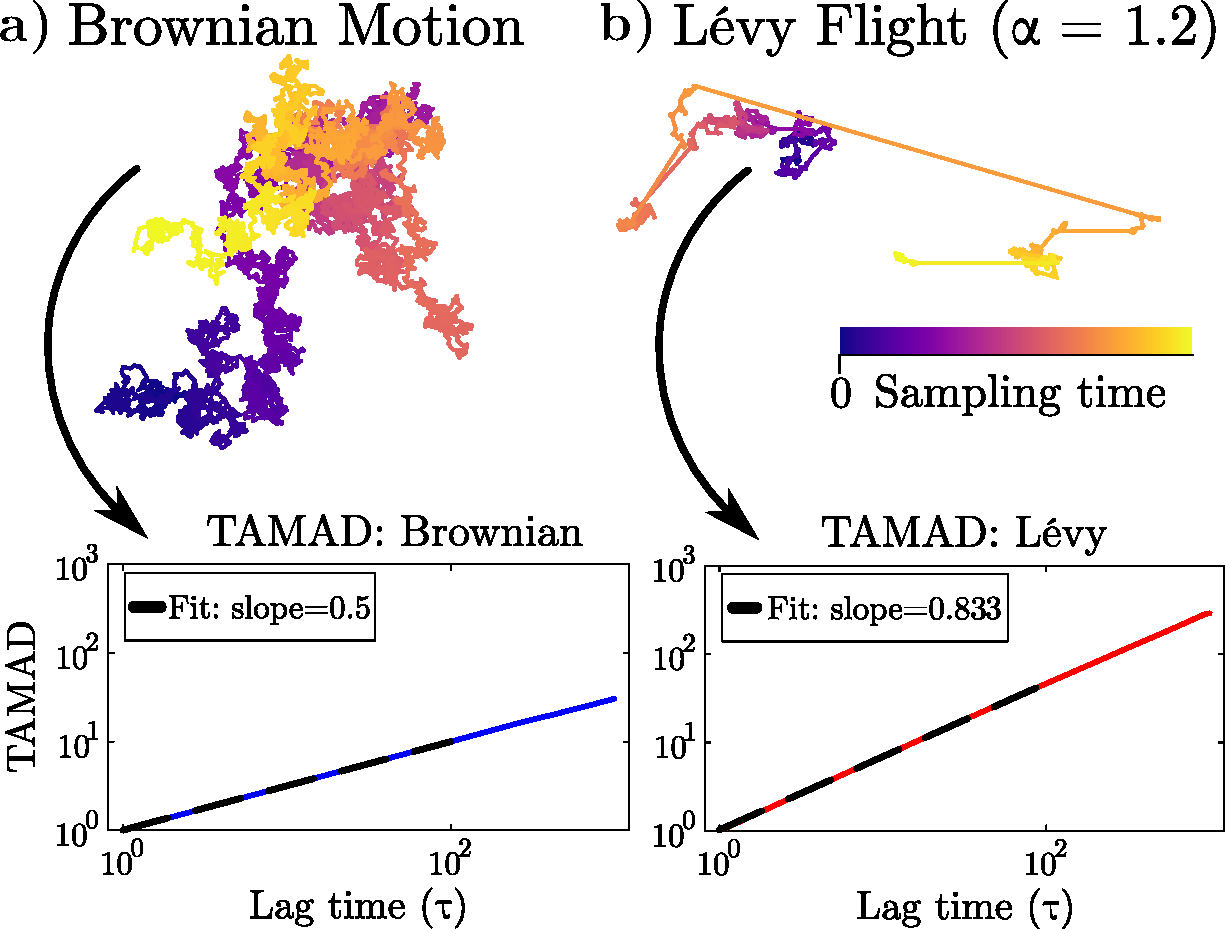
\includegraphics[width=0.8\linewidth]{figures/BvL.pdf}
	\caption{\textbf{Schematic representations of stochastic motion and their respective diffusion.} \textbf{a)} Schematic representation of a 2D Brownian motion, along with its time-averaged mean absolute displacement (TAMAD), which is the $q=1$ mean fractional displacement as in \cref{eq:MFD}. Normal diffusion is here present as a power law slope of exponent $1/2$, giving diffusive exponent $\beta=1$ as defined in \cref{eq:MFD}. \textbf{b)} Schematic of a superdiffusive 2D Lévy flight with characteristic exponent of $\alpha=1.2$, and a MAD slope of $0.833$ corresponding to the theoretical superdiffusive coefficient $\beta= 2/\alpha = 5/3$.}
	\label{fig:brownian_vs_levy}
\end{figure}
To mathematically capture the intermittent, scale-free nature of visual search, we turn to the Lévy flight: a superdiffusive stochastic process that permits close analysis, due to it's very foundational mathematical definition. Here, the Lévy flight $L_t^{\alpha}$ is a stochastic process defined through it's increments being drawn from a heavy tailed symmetric $\alpha$-stable distribution (a $\mathcal{S}\alpha\mathcal{S}$ distribution), where $\alpha$ is called the characteristic exponent and relates to the exponent of the distributions powerlaw tails. $\mathcal{S}\alpha\mathcal{S}$ distributions describe the limit of summation of i.i.d infinite-variance variables, as a result of the generalised central limit theorem, making them ideal to describe a universality class of superdiffusive processes. The $\alpha$ value defining a particular $\mathcal{S}\alpha\mathcal{S}$ distribution is a result of the asymptotic power-law tail of the density function, with the probability density function following $p(x) \propto |x|^{-1-\alpha}$. As a result, the Lévy flight $L_t^{\alpha}$ after time $t$ is defined by its fractional scaling properties and alpha-stable statistics
\begin{equation} \label{eq:levy_noise}
	L_t \stackrel{d}{=} t^{1/\alpha} L_1, \ \ L_1 \sim \mathcal{S}\alpha\mathcal{S}
\end{equation}
where $\stackrel{d}{=}$ denotes equal in distribution. In the limit $\alpha \rightarrow 2$, the Lévy flight reduces to a scaled Brownian Motion $L_t^{\alpha \rightarrow 2} = \frac{1}{\sqrt{2}}W_t$. If $1 < \alpha < 2$ the variance of $L_t^{\alpha}$ diverges and has mean 0, whereas if $0 < \alpha \leq 1$, then both the variance and mean diverge. In analysing the distribution of a Lévy flight, one must generalise the standard Langevin Fokker-Planck equation (\ref{eq:overdamped-fokkerplanck}) to the Lévy motion using fractional calculus to capture the nonlocal transport of the particle. The details of such an analysis are beyond this thesis, however the fractional Fokker-Planck equation is the tool used to understand the superdiffusion, nonlocality, and scale-free behaviour of trajectories of Lévy flights (see the appendices to \cite{qi_fractional_2022}). Many of the simple analytic properties of the Brownian motion are no longer true of a Lévy flight. Notably, since these flights have infinite variance in steps sizes, the mean squared displacement diverges. Thus their superdiffusion is better measured using an extension of MSD to fractional absolute displacements, through the definition of the moment spectrum function $\lambda(q)$ as in \cite{vilk_strong_2025}:
\begin{equation}\label{eq:MFD}
	\langle \| \Delta \textbf{x}(t) \| ^ q \rangle \propto t^{\lambda(q)}, \ \ q > 0
\end{equation}
where $q$ is the order of the fractional absolute displacement, and the power law slope will converge for an $\alpha$-Lévy flight to $\lambda(q) = q/\alpha$ when $q < \alpha$. As such, for Lévy flights with exponents $\alpha > 1$ superdiffusion is well-characterised by the mean absolute displacement, where $q=1$ in \cref{eq:MFD}.

Importantly, trajectories of a Lévy flight are no longer continuous. Instead, such trajectories are called \textit{càdlàg} (continue à droite, limite à gauche) with respect to time, which describes functions which are right continuous with well-defined left limits \cite{van_den_Bosch}. Thus, we say that since all such trajectories produced from a Lévy flight are càdlàg, the Lévy flight itself is called a càdlàg process. Càdlàg processes have been widely studied in the context of mathematics, economics, and physics, and their properties are well understood \cite{soulier2022-ge, Borkar1995}. It has been shown that Lévy flights are semimartingales, and are well interpreted in integration \cite{van_den_Bosch}. Importantly, it follows from the Lévy-Itô decomposition theorem that a Lévy flight can be decomposed as the sum of two processes \cite{Kyprianou2014}:
\begin{enumerate}
	\item A compound Poisson process of large jumps with $\| \Delta \textbf{x} \| > 1$. Such jumps are exponentially distributed in time, and there are almost surely a finite number in any finite time period.
	\item A square-integrable martingale (mean 0) jump process with $\| \Delta \textbf{x} \| < 1$. This process is then finite-variance, and as such is subject to the central limit theorem, meaning that under temporal coarse graining it approaches a Brownian motion.
\end{enumerate}
This division is useful in analysing the process in the context of nonlocal stochastic exploration in Lévy flights, which is modelled by the compound Poisson process of large jumps $|\Delta \textbf{x}| > 1$, and the local exploitation dynamics modelled by the square-integrable martingale of small jumps $|\Delta \textbf{x}| < 1$. In the context of visual searching, such a division naturally inspires the division between large jumps of attention, and periods of prolonged attention. As such, we are interested in why such superdiffusive scale-free dynamics may have a powerful in computational advantage in exploring an abstract unknown landscape.

%\subsection{Nested oscillations}

%%% 1.2 Abstract Computation
\section{Probabilistic computation}\label{sec:comp_sampling}
The stochastic dynamical exploration of an information landscape is a powerful paradigm of general computation, and is known as probabilistic computation. Such a landscape in this context is a representation of a target probability distribution. Sampling processes represent and evaluate these distributions through the efficient production of informative stochastic samples. Uncertain, high-dimensional, and ambiguous inference problems require efficient and accurate characterisations of target distributions. Sampling methods aim to draw sampled independently from a target distribution. This paradigm has become widely utilised in machine learning and statistics, where generative models learn patterns from sparse samples of large multivariate distributions inferred from observational data \cite{delacour_neural_1997, cranmer_advances_2023}. This framework has recently gained significant traction as a basic scheme to describe biological computation. The variability in firing patterns of neural populations would thus maintain an internal model of perceptual uncertainty and evolving understanding, giving a functional role to chaotic neural activity \cite{rao_predictive_1999, koch_predicting_1999, lange_bayesian_2020}. This section outlines the paradigm of neural sampling as an interpretation of the variability in neuron firing patterns and visual search gaze trajectories (\cref{subsec:neur_sampling}) as well as their extension to describe visual searching as a sampling process (\cref{subsec:visual_sampling}).
%\subsection{Active perception}\label{subsec:active_inf}
%The dominant framework in modern computational neuroscience is that of the Bayesian brain. Karl Friston, the most cited neuroscientist \cite{Bohannon2016-kp}, developed this framework, and shifted the view of the perceptual loop of the brain. Friston's theory of active inference described perception through inferring and generating top-down sensory predictions of the world, and carrying back the bottom-up errors from that perception. This development brought a strong shift in the literature, ``marking a watershed between 20th-century thinking about the brain as a glorious stimulus–response link and more constructivist 21st century perspectives that emphasized an active sampling of the sensory world'' (\cite{friston_does_2018} pg. 1019). The active inference model of an updating internal mental state filled the explanatory gap in the understanding of the functional role of many key feedback mechanisms in the brain \cite{rao_predictive_1999, koch_predicting_1999}, and went on to yield successful predictions of how the brain optimally deciphers noisy multimodal sensory inputs \cite{kording_bayesian_2004}, as well as provide rigorous frameworks to base probabilistic computation in the brain \cite{lange_bayesian_2020}. There has recently been opposition to the general framework of the Bayesian brain and active inference \cite{mangalam_myth_2025}. Much of the arguments against such a framework arise from the philosophy of science, where active inference in perception may be supported post-hoc through ``just so'' definitions of priors \cite{mangalam_myth_2025, bowers_bayesian_2012}. It is therefore important to understand the Bayesian brain hypothesis as a normative framework from which to build falsifiable, understandable, and biologically plausible theories of neural computation.

\subsection{Neural sampling}\label{subsec:neur_sampling}
The framework of neural sampling posits this paradigm that the variability of cortical neural responses is an important functional feature of biological computation. Otherwise regarded as noise, stochastic neural activity patterns are thus presented as samples drawn from a posterior distribution over possible sensory interpretations \cite{orban_neural_2016, NIPS2002_a486cd07}. The neural sampling hypothesis has been shown to perform and predict network-level empirical patterns of neural activity in the V1, and recently by Terada and Toyoizumi in biologically realistic cortical networks, better than alternative theories \cite{NIPS2002_a486cd07, ujfalussy_sampling_2022, terada_chaotic_2024, orban_neural_2016}. Perceptual uncertainty is then encoded by the variability of these cortical responses across time and across multiple trials, with higher uncertainty reflected in wider response distributions \cite{NIPS2002_a486cd07, delacour_neural_1997, orban_neural_2016}. Neural sampling thus provides an interpretation for the way the brain navigates uncertainty at the fundamental scale of neural computation.

Studies into neural sampling show that variability is not strictly a result of explicit stochastic noise, as traditionally believed. Instead, recent work demonstrates that strongly recurrent, balanced inhibitory-excitatory deterministic neural networks can generate the high-dimensional variability which stochastic models are built to capture \cite{terada_chaotic_2024, NIPS2002_a486cd07}. Terada and Toyoizumi link this sampling of a posterior distribution to Bayesian learning through training a recurrent network to sample static features and dynamic trajectories, generalising learned priors to novel, uncertain environments through biologically plausible learning \cite{terada_chaotic_2024}. Further biologically plausible implementations of such Bayesian sampling are energy-based models (EBMs) which suggest that fast-spiking interneurons can estimate the local partition function to enable fast, localised sampling dynamics \cite{dong_neural_nodate}. The sampling hypothesis has thus given a convincing theory of biological neural computation, with testable and well-supported evidence that neural variability has an important functional role in computation \cite{orban_neural_2016, ujfalussy_sampling_2022}. Traditional Gaussian and Poisson noise models representing these stochastic network dynamics inherently correspond to continuous struggle to capture the full dynamics of complex interconnected inhibitory-excitatory (IE) biological neuronal network \cite{koren_efficient_2025, kilgore_biologically-informed_2025, song_training_2016}. Further study into the dynamics of these IE networks has thus motivated further functional models of neural activity.

\subsubsection*{Fractional neural sampling}

%In reality, neural activity has been found to exhibit structure across multiple spatial and temporal scales, often described by scale-free statistics \cite{boonstra_scale-free_2013, he_scale-free_2014, he_temporal_2010, jiao_biologically_2026, jones_scale-free_2023, lin_scale-free_2016, mashour_conscious_2020, roberts_heavy_2015, zhang_heavy-tailed_2025}. This observation, together with the neural sampling hypothesis, motivates the design and theory of Fractional Neural Sampling (FNS) \cite{qi_fractional_2022}. FNS describes the complex spatiotemporal dynamics of spiking neural circuits, where localised activity patterns propagate through superdiffusive Lévy flights. Such Lévy flight dynamics of the centre of mass of firing spikes $\textbf{x}_t$ with a Langevin equation driven by Lévy noise and coupled to a momentum term $\textbf{p}_t$, which we shall call the FNS equations of motion,
%
%\begin{equation}
%\label{eq:fns}
%\begin{aligned}
%	d\textbf{x}_t &= \gamma b(\textbf{x}_t)dt + \beta \textbf{p}_t dt + \gamma^{1/\alpha} dL_t^{\alpha}, \\
%	d\textbf{p}_t &= \beta b(\textbf{x}_t) dt
%\end{aligned}
%\end{equation}
%
%where $\textbf{x}_t$ is the (usually 2 dimensional) vector of position, $\textbf{p}_t$ is a generalised auxiliary variable analogous to a momentum of the same dimensionality, $\beta > 0$ is a parameter defining the strength of coupling between $\textbf{p}_t$ and $\textbf{x}_t$, $\gamma > 0$ is the noise strength parameter, $ 0 < \alpha \leq 2$ is the Lévy tail exponent, and $dL_t^{\alpha}$ is the Lévy stable noise drawn from a $\mathcal{S}\alpha\mathcal{S}$ distribution. The term $b(\textbf{x}_t)$ captures a deterministic gradient term in the dynamics, defined such that the invariant distribution of $\textbf{x}_t$ after long time $t$ approaches the target distribution sampled, $\pi(\textbf{x})$. The exact expression for $b_{\alpha}(\textbf{x})$ is derived in \cite{qi_fractional_2022}, and approaches the gradient of the logarithm of the density as $\alpha \rightarrow 2$, with the full form for any $ 0 < \alpha \leq 2$ given in terms of the $\alpha-2$-order Riesz fractional derivative $\mathcal{D}^{\alpha - 2}_{\textbf{x}}$ as
%
%\begin{equation}\label{eq:full_drift}
%	b_{\alpha}(\textbf{x}) = \frac{\mathcal{D}^{\alpha - 2}_{\textbf{x}}[\pi(\textbf{x}) \partial_{\textbf{x}} \ln\pi(\textbf{x})]}{\pi(\textbf{x})}
%\end{equation}
%with the useful local approximation, which becomes exact at $\alpha=2$,
%\begin{equation}\label{eq:drift_approx}
%    b_{\alpha}(\textbf{x}) \approx c_{\alpha} \nabla_{\textbf{x}} \ln \pi(\textbf{x}), \qquad c_{\alpha} = \frac{\Gamma(\alpha - 1)}{\Gamma(\frac{\alpha}{2})^2}
%\end{equation}

The FNS dynamics are called fractional, as the non-local dynamics of their distribution require fractional calculus to describe such spatial superdiffusion in Lévy flights \cite{tarasov_general_2021}. The theory of FNS thus unifies the scale-free nonlocal dynamics of neural firing patterns with the neural sampling framework derived from the ideal Bayesian scheme of active inference. The critical advantage of FNS over other standard continuous random walks is its ability to efficiently sample complex, multimodal probability distributions with far-apart modes—likely a major feature of processed natural environments replete with multiple distinct salient features. While Brownian-motion-based samplers typically remain trapped in local modes due to high potential energy barriers, the heavy-tailed, large jumps inherent in FNS enable the neural sampler to adaptively and freely switch between multiple modes \cite{neal_sampling_1996, latuszynski_mcmc_2025, simsekli_fractional_nodate, metzler_random_2000}. Furthermore, the generality of the FNS description permits the application of FNS equations of motion to gaze dynamics, as the motion of the eyes are driven by an IE neural circuit which is expected to keep key features of the FNS model invariant, such as superdiffusion, heavy-tailed statistics, and nonlocal interactions.

\subsection{Visual sampling}\label{subsec:visual_sampling}
This thesis presents visual search tasks as such a paradigm where a sampling model is well motivated, and driven by the underlying neural sampling process as well. The visual system is evolved to actively and efficiently process noisy information and evidence from the external world, and plan future search paths to gather further noisy evidence \cite{Renninger2005-ee, renninger_where_2007, najemnik_optimal_2005, bujia_modeling_2022}. In the context of visual searching, visually interesting targets with \textit{saliency} as the equivalent of the target landscape, and where the information is located in a target image. Here, saliency is equivalent to the Boltzmann log-likelihood potential from the probability distribution of fixations $p(\textbf{x})$
\begin{equation}\label{eq:saliency}
	S(\textbf{x}) = -\log(p(\textbf{x}))
\end{equation}
where visual search paths are most likely to be drawn to is a common technique whic \cite{Bruce_2009_Saliency}. As such, undirected visual searching of an image will show the areas most salient to the brain, allowing insight into the computational sampling mechanism of the visual system. In particular, search tasks require sophisticated integration of the cost and expected information gain of decisions, which invites fruitful decision analysis \cite{Wedel_2023}. Empirical experiments show that eye movements show good agreement with greedy local information maximising fixations, given well-motivated visual sensitivity based on human physiology \cite{Radulescu_2026, najemnik_optimal_2005, renninger_where_2007}.

%%This dynamical switching provides a functional explanation for the bimodality of estimate distributions observed in human perceptual switching and visual perception inference.
%\subsection{Markov Chain Monte Carlo methods}\label{subsec:MCMC}
%This view of neural- and visual sampling of a target distribution motivates analogy to a foundational set of methods in machine learning. Markov Chain Monte Carlo (MCMC) methods have become the algorithmic basis for generating samples from target distributions in rigorous Bayesian inference in machine learning \cite{cranmer_advances_2023, latuszynski_mcmc_2025, speagle_conceptual_2020, andrieu_particle_2010}. MCMC operates by constructing a Markov chain, where the transition matrix is calculated such that the equilibrium distribution of samples is the desired target distribution. In the context of neural computation, biological circuits are often modelled as implementing continuous-time variants of MCMC sampling of neural population targets, most notably through Langevin sampling and Hamiltonian Monte Carlo (HMC) \cite{latuszynski_mcmc_2025, betancourt_conceptual_2018}. Langevin sampling dynamics utilise local gradient information from the probability landscape, combined with Gaussian white noise, to explore the state space over time. Such dynamics are identical to the Langevin system studied in statistical physics, described in \cref{eq:langevin}, where $V(\textbf{x}) = - \log(\pi(\textbf{x}))$ is the potential function over parameters $\textbf{x}$ required yielding a distribution $\pi(\textbf{x})$ of samples. Despite their ubiquity, traditional MCMC methods encounter severe theoretical and practical limitations when exploring unknown, heavy-tailed, and/or multimodal target distributions. Standard Langevin and HMC dynamics are driven by continuous Brownian and Hamiltonian motion respectively, and the traversal of low-probability regions, equivalent to dynamical energy barriers, becomes exponentially slow. Consequently, the mean exit time for the sampler to leave one mode and discover another grows exponentially with the modal separation distance \cite{latuszynski_mcmc_2025}. To accelerate this sluggish exploration, algorithms often introduce auxiliary momentum variables to drive global landscape traversal, as in the FNS equations of motion \ref{eq:fns}. However, even with momentum-based acceleration, traversing deep energy valleys remains highly inefficient \cite{latuszynski_mcmc_2025, neal_sampling_1996, betancourt_conceptual_2018}. The nonlocal dynamics introduced in fractional sampling are one branch of research into how rapid mixing of samples in complex distributions can be achieved without the need for nontrivial parameter tuning and knowledge of the distribution of interest. For instance, fractional algorithms based on Hamiltonian Monte Carlo sampling and second-order Langevin sampling with a momentum variable have been briefly developed and explored \cite{simsekli_fractional_nodate, ijcai2018p419, qi_fractional_2022, oechsler_levy_2024, behme_levy_2026}. Importantly, FNS dynamics over a probability landscape yield a mean exit time between modes which scales linearly rather than exponentially with separation \cite{qi_fractional_2022}. FNS dynamics thus demonstrate a profound computational advantage for efficient biological inference through it's background as an effective sampling algorithm.
